\section{误差与计算成本}
\label{sec:sgdb-cost}

本章已经出现了很多方法，每一种都有自己的误差界和成本描述。它们能不能放在一起比较？回答这个问题，先要固定三件事：要最小化哪个目标，算法返回什么，用什么量计算成本。本节依次讨论评价对象、总计算成本，以及当输入的数据发生变化时算法的有限步响应。

\subsection{误差的评价对象}
\label{sec:sgdb-error-objects}

\paragraph{量与返回点的配对}
一个收敛结论由两部分组成：度量什么量，度量哪个点。常用的量有目标差、到最小点的距离、梯度范数或邻近残差；常用的返回点有最后一点、平均点和随机返回点。量和点的配对不能互换，表~\ref{tab:sgdb-error-pairing}列出常见的配对。

\begin{BookInlineTable}
  \centering
  \caption{常见的误差量与返回点的配对。条件只列出主要假设，具体常数和步长以相应结论为准。}
  \label{tab:sgdb-error-pairing}
  \begin{tabular}{lll}
    \toprule
    误差量 & 返回点 & 主要条件\\
    \midrule
    期望目标差 & 加权平均点 & 凸\\
    期望目标差 & 最后一点 & 强凸\\
    到最小点的距离 & 最后一点 & 强凸\\
    平方梯度范数 & 按权重随机返回 & 光滑非凸\\
    邻近残差 & 按权重随机返回 & 复合目标\\
    \bottomrule
  \end{tabular}
\end{BookInlineTable}

配对的差别可以在贯穿例上看见。常步长$\alpha=0.1$时，随机梯度下降的最后一点的期望目标差趋于$0.528$，不随轮数继续下降。模拟$20$万条路径，后$2000$轮的平均点的期望目标差约为$0.0024$，比最后一点小两个多量级。平均减小了噪声，但关于平均点的界不能直接移用到某个单独的迭代点上。

\paragraph{期望保证与概率保证}
上面的误差界都是期望。期望小不等于每次运行都小。若$Z\geq0$是目标差，$\mathbb{E}Z\leq\varepsilon$，由Markov不等式，对任意$\delta\in(0,1)$，
\begin{equation}
 \mathbb{P}\Bigl(Z\geq\frac{\varepsilon}{\delta}\Bigr)\leq\delta .
 \label{eq:sgdb-markov}
\end{equation}

比如$\mathbb{E}Z\leq0.01$，只能得到目标差超过$0.1$的概率不超过$0.1$。这里$\varepsilon/\delta$随$\delta$变小放大得很快。更强的高概率保证需要读数的尾部条件，例如有界或次高斯，并使用鞅集中不等式，推导要用到鞅的工具，这里只说明它与期望保证的区别。

路径的长期性质是另一个问题，例如一条路径是否几乎必然收敛，这类结论依赖步长条件和鞅收敛定理，属于前面提到的长期路径分析。有限步的期望界不能回答这个问题。

\paragraph{各类误差进入递推的位置}
本章遇到的误差进入递推的不同位置。条件噪声进入二次项，贡献$\sigma^2$乘以步长的相应幂次，能靠减小步长或增大批量压低。系统偏差进入一次项，贡献的$B^2$不随步长变小。近似求解的误差与偏差类似，由内层精度决定。

这些都是\term{优化误差}（optimization error），针对的是给定的目标。如果目标是由一批样本构造的有限和，而真正关心的是总体上的目标，那么还有一部分由样本有限造成的差距。这部分属于统计误差，优化再精确也不能消除，分析它需要样本数和分布条件。优化误差不能代替统计误差，反过来也一样。

\subsection{总计算成本}
\label{sec:sgdb-total-cost}

\paragraph{统一单位}
比较方法之前，先把计量单位统一下来。常用的单位有样本梯度读取次数、参数更新次数、完整遍历次数。一次全梯度是$N$次样本梯度读取；一轮批量大小为$b$的小批量是$b$次读取、一次更新。此外要把快照、梯度表、矩阵分解、邻近求解、同步统计这些额外工作计入。

下面的估计都假定目标在同一种归一化下，要求同一个精度$\varepsilon$，略去常数因子。设$f$是$N$项的平均，强凸常数$\mu$，整体光滑常数$L$，逐项光滑常数最大值$L_{\max}$，$\kappa_{\max}=L_{\max}/\mu$，读数方差$\sigma^2$。

\begin{BookInlineTable}
  \centering
  \caption{强凸有限和目标上达到目标差$\varepsilon$的样本梯度读取量，略去常数因子。}
  \label{tab:sgdb-cost-table}
  \begin{tabular}{lll}
    \toprule
    方法 & 读取量 & 额外状态\\
    \midrule
    全梯度下降 & $N\kappa\ln(1/\varepsilon)$ & 无\\
    随机梯度下降 & $\sigma^2/(\mu\varepsilon)$ & 无\\
    SVRG & $(N+\kappa_{\max})\ln(1/\varepsilon)$ & 一个快照\\
    SAGA & $(N+\kappa_{\max})\ln(1/\varepsilon)$ & 梯度表，$N$份\\
    \bottomrule
  \end{tabular}
\end{BookInlineTable}

用具体数比较。取$N=1000$，$\kappa=\kappa_{\max}=100$，$\sigma^2/\mu=1$。

当$\varepsilon=10^{-3}$时，$\ln(1/\varepsilon)\approx6.9$，全梯度下降、随机梯度下降和SVRG的读取量分别是
\[
 6.9\times10^{5},\qquad 1000,\qquad 7.6\times10^{3},
\]
随机梯度下降最便宜。当$\varepsilon=10^{-6}$时，$\ln(1/\varepsilon)\approx13.8$，三个读取量变成
\[
 1.4\times10^{6},\qquad 10^{6},\qquad 1.5\times10^{4},
\]
SVRG的读取量比随机梯度下降少约$60$倍。结论是：用什么方法取决于要求的精度，低精度时常步长的简单方法足够，高精度时方差减小的方法更划算。

\paragraph{按不同单位，排序不同}
图~\ref{fig:sgdb-cost-units}在同一个最小二乘问题上用两种单位画出四种方法。按参数更新次数，全梯度下降明显最快，因为每次更新读了全部$200$项。按样本读取量，全梯度下降落到后面，SAGA和随机梯度下降早期下降最快。只按外层轮数排序，或者只按更新次数排序，都会得出不同的结论。

\begin{BookInlineFigure}
  \centering
  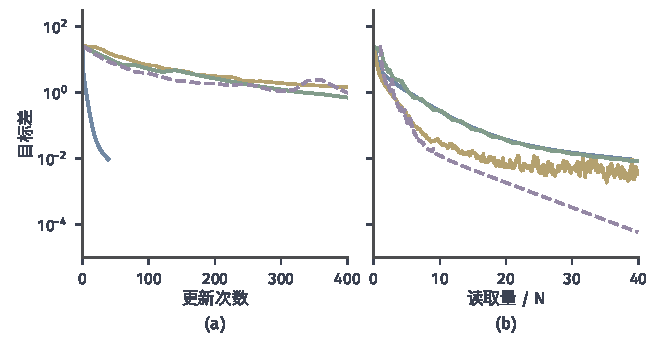
\includegraphics[width=112mm]{figures/05-optimization/05-stochastic-optimization/matplotlib/sgdb-cost-units/figure.pdf}
  \caption{同一个问题按不同单位的进展，有限和最小二乘加平方惩罚，$N=200$，$n=10$，$\gamma=0.1$。蓝线是步长$1/L$的全梯度下降，黄线是常步长随机梯度下降，绿线是SVRG，紫色虚线是SAGA。(a)横轴是参数更新次数。(b)横轴是样本读取量除以$N$，SVRG的快照和控制变量都计入读取量，SAGA的梯度表初始化也计入。}
  \label{fig:sgdb-cost-units}
\end{BookInlineFigure}

\paragraph{批量、微批量与历史更新的计时}
计时单位在调度中也要说明。步长调度按更新次数、样本读取量还是遍历次数推进，不同的实现可能相差一个批量大小的倍数。把一个批量拆成微批量累积梯度时，读取量不变，但更新次数减少；若统计量（比如批量内的归一化）按微批量更新，就要规定它的计时。

减少更新次数是否值得增加单步工作，取决于这次工作能否并行、读取是否昂贵、更新本身的成本。计算结论应写成“在某某单位下，某方法达到某精度需要多少”，不能只说某方法更快。

\subsection{样本替换的有限步响应}
\label{sec:sgdb-stability}

\paragraph{问题}
前面都固定了目标。现在换一个问题：两份数据只相差一个样本，让同一个算法在两份数据上运行，输出相差多少？这刻画的是算法这个从数据到输出的映射对单个样本有多敏感，称为\term{算法稳定性}（algorithmic stability）。

设目标$f$由$N$项平均而成，另一份数据的目标$\tilde f$只把第$k$项换成$\tilde f_k$，其余项相同。两次运行使用相同的初值、相同的步长序列，以及\emph{相同的}下标路径$i^{(0)},i^{(1)},\ldots$，得到$\bm{x}^{(t)}$和$\tilde{\bm x}^{(t)}$。这种做法称为耦合，它把抽样噪声的影响去掉，图~\ref{fig:sgdb-coupling}展示了它的结构：差异只在抽到第$k$项时产生。

\begin{BookInlineFigure}
  \centering
  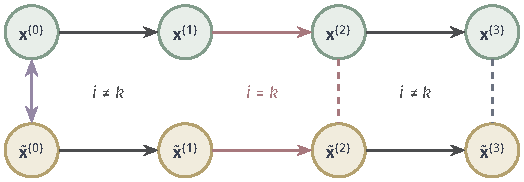
\includegraphics[width=88.74mm]{figures/05-optimization/05-stochastic-optimization/tikz/sgdb-coupling/figure.pdf}
  \caption{两次耦合运行。两条轨迹起点相同（紫色）。下标$i\neq k$时，两边用同一项更新，只传播已有差异；$i=k$时（红色箭头），两边用不同的项更新，新差异在此注入。}
  \label{fig:sgdb-coupling}
\end{BookInlineFigure}

\paragraph{用贯穿例计算}
取贯穿例，把第$3$项$f_3=\frac32(x-3)^2$换成$\tilde f_3=\frac32x^2$，也就是$b_3$从$3$变成$0$。起点都是$2$，$\alpha=0.1$，读取顺序为第$3,1,2$项，其中第一轮抽到被替换的项。两条轨迹依次是
\[
 \begin{aligned}
 x^{(1)}&=2.3, & \tilde x^{(1)}&=1.4, & \lvert x-\tilde x\rvert&=0.9,\\
 x^{(2)}&=1.77, & \tilde x^{(2)}&=0.96, & \lvert x-\tilde x\rvert&=0.81,\\
 x^{(3)}&=1.416, & \tilde x^{(3)}&=0.768, & \lvert x-\tilde x\rvert&=0.648.
 \end{aligned}
\]

第一轮两边的读数分别是$-3$和$6$，注入的差异是$0.1\cdot9=0.9$。后两轮用相同的项，$a_i=1,2$，差异分别乘以$1-\alpha a_i=0.9$和$0.8$，没有放大。下面的分析把这两种情形一般化。

\paragraph{传播：梯度步的非扩张}
先看未抽到被替换项的一步。两边用同一个函数走一步，距离不增加，这由下面的引理保证。这里为了证明简短，假定函数二阶连续可微。

\begin{lemma}[梯度步的非扩张与压缩]
\label{lem:sgdb-nonexpansive}
设$\phi$二阶连续可微，$\mu_0\bm{I}\preceq\nabla^2\phi\preceq L\bm{I}$，$\mu_0\geq0$。若$0<\alpha\leq2/(L+\mu_0)$，则对任意$\bm{x},\bm{y}$，
\begin{equation}
 \bigl\lVert\bigl(\bm{x}-\alpha\nabla\phi(\bm{x})\bigr)-\bigl(\bm{y}-\alpha\nabla\phi(\bm{y})\bigr)\bigr\rVert_2\leq(1-\alpha\mu_0)\lVert\bm{x}-\bm{y}\rVert_2 .
 \label{eq:sgdb-nonexpansive}
\end{equation}
\end{lemma}

\begin{proof}
由微积分基本定理，
\[
 \nabla\phi(\bm{x})-\nabla\phi(\bm{y})=\bm{A}(\bm{x}-\bm{y}),\qquad
 \bm{A}=\int_0^1\nabla^2\phi\bigl(\bm{y}+s(\bm{x}-\bm{y})\bigr)\,\mathrm{d}s .
\]

$\bm{A}$对称且$\mu_0\bm{I}\preceq\bm{A}\preceq L\bm{I}$。于是左端等于$\lVert(\bm{I}-\alpha\bm{A})(\bm{x}-\bm{y})\rVert_2$，矩阵$\bm{I}-\alpha\bm{A}$的特征值落在$[1-\alpha L,1-\alpha\mu_0]$内。条件$\alpha\leq2/(L+\mu_0)$保证$\alpha L-1\leq1-\alpha\mu_0$，所以这些特征值的绝对值不超过$1-\alpha\mu_0$，由此得到结论。
\end{proof}

\paragraph{注入与传播的合成}
差异只在抽到第$k$项时产生，每一步的概率是$1/N$。下面的定理把注入和传播合成一个界。

\begin{theorem}[样本替换下的期望参数距离]
\label{thm:sgdb-stability}
设每个$f_i$与$\tilde f_k$二阶连续可微，满足$\bm{0}\preceq\nabla^2\preceq L\bm{I}$。下标独立均匀抽取，确定的步长满足$0<\alpha^{(t)}\leq2/L$。设在两条轨迹访问的点上，被替换的两项梯度满足
\begin{equation}
 \lVert\nabla f_k(\bm{x}^{(t)})\rVert_2\leq G,\qquad \lVert\nabla\tilde f_k(\tilde{\bm x}^{(t)})\rVert_2\leq G .
 \label{eq:sgdb-stability-condition}
\end{equation}
则
\begin{equation}
 \mathbb{E}\lVert\bm{x}^{(T)}-\tilde{\bm x}^{(T)}\rVert_2\leq\frac{2G}{N}\sum_{t=0}^{T-1}\alpha^{(t)} .
 \label{eq:sgdb-stability}
\end{equation}
\end{theorem}

\begin{proof}
记两条轨迹的距离为
\[
 \delta^{(t)}=\lVert\bm{x}^{(t)}-\tilde{\bm x}^{(t)}\rVert_2,\qquad\delta^{(0)}=0.
\]

若$i^{(t)}\neq k$，两条轨迹用同一个$f_i$走一步，由引理~\ref{lem:sgdb-nonexpansive}（$\mu_0=0$），
\[
 \delta^{(t+1)}\leq\delta^{(t)} .
\]

若$i^{(t)}=k$，由三角不等式和式~\eqref{eq:sgdb-stability-condition}，
\[
 \delta^{(t+1)}\leq\delta^{(t)}+\alpha^{(t)}\bigl(\lVert\nabla f_k(\bm{x}^{(t)})\rVert_2+\lVert\nabla\tilde f_k(\tilde{\bm x}^{(t)})\rVert_2\bigr)\leq\delta^{(t)}+2\alpha^{(t)}G .
\]

下标与历史独立，后一种情形的条件概率是$1/N$，所以
\[
 \mathbb{E}\bigl[\delta^{(t+1)}\mid\mathcal{F}^{(t)}\bigr]\leq\delta^{(t)}+\frac{2\alpha^{(t)}G}{N}.
\]

取全期望，对$t=0,\ldots,T-1$累加，得到式~\eqref{eq:sgdb-stability}。
\end{proof}

这个界的结构是：每步以概率$1/N$注入不超过$2\alpha^{(t)}G$的差异，注入后的差异不再放大。若每项还$\mu_0$强凸，$\mu_0>0$，$\alpha\leq2/(L+\mu_0)$，引理给出的压缩因子就进入递推，常步长下
\[
 \mathbb{E}\delta^{(t+1)}\leq(1-\alpha\mu_0)\mathbb{E}\delta^{(t)}+\frac{2\alpha G}{N},
\]
它的极限不超过$2G/(N\mu_0)$，界不再随$T$无限增长。图~\ref{fig:sgdb-stability-run}(b)显示了实际平均距离与两条界：实际距离上升到约$0.04$后回落并稳定，远低于两条上界。上界偏保守的一个原因是$G$取了路径上的最大值，而实际注入的差异通常小于$2\alpha G$。

\begin{BookInlineFigure}
  \centering
  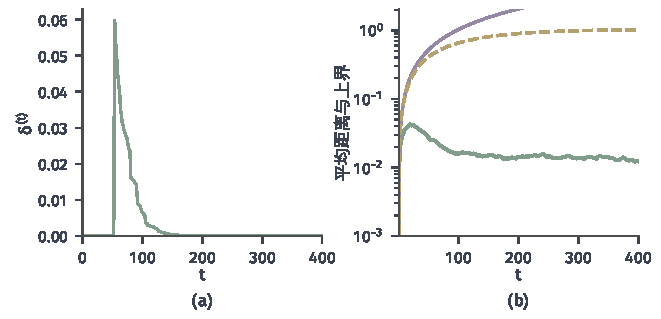
\includegraphics[width=112mm]{figures/05-optimization/05-stochastic-optimization/matplotlib/sgdb-stability-run/figure.pdf}
  \caption{样本替换的有限步响应，平方损失加平方惩罚的$N=100$项平均，$\gamma=0.2$，常步长$1/L_{\max}$，第$1$项被替换。(a)一条耦合路径上的距离$\delta^{(t)}$：抽到被替换项时跳起，之后逐渐压缩。(b)$1500$对路径的平均距离（绿），式~\eqref{eq:sgdb-stability}的非扩张界（紫）与利用强凸的压缩界（黄色虚线）。}
  \label{fig:sgdb-stability-run}
\end{BookInlineFigure}

\paragraph{结论的适用范围}
逐项的条件要逐一核对。这里要求的是每一项凸且光滑，只有平均目标凸是不够的，否则未抽到被替换项的那一步也可能拉开距离。凸性和步长决定传播：目标不凸时，梯度步可以把差异放大到$1+\alpha L$倍；步长超过$2/L$时，即使凸函数的梯度步也可能扩张。梯度界$G$只需要在实际访问的点上成立；对最小二乘这样的目标，它依赖轨迹所停留的区域。去掉二阶可微条件时，凸$L$光滑函数的梯度步仍然非扩张，证明需要梯度的余强制性，篇幅较长，读者可查阅\scite{hardt2016sgd}。

式~\eqref{eq:sgdb-stability}说的是参数的距离。要把它转成损失的变化，还需要损失对参数的定量控制：若损失关于参数$K$-Lipschitz，则损失之差不超过$K\lVert\bm{x}^{(T)}-\tilde{\bm x}^{(T)}\rVert_2$。这是另一个独立的条件。从算法的输出差异到统计泛化结论，还要有样本分布和数据生成假设，这部分不在有限步优化的范围内。
